\documentclass{llncs}
\usepackage{llncsdoc}
\usepackage[utf8]{inputenc}
\usepackage[compatibility=false]{caption}
\usepackage{amsmath}
\usepackage{amsfonts}
\usepackage{amssymb}
\usepackage{bbm}
\usepackage[ruled,vlined]{algorithm2e}
\usepackage{graphicx}
\usepackage{caption}
\usepackage{subcaption}
\usepackage{dsfont}
\author{Amit Wolfenfeld\inst{1}}
\institute{Technion}
\title{Title}

\begin{document}
\maketitle

\begin{abstract}
The Dueling Bandits setting is an online learning framework in which actions are restricted to stochastic comparisons between pairs of strategies.
It models settings were absolute rewards are difficult to estimate but pairwise preferences are readily available. This set-up is extremely relevant, for example, in the world of internet marketing.
In this paper we propose several new methods for the Dueling Bandit Problem. Our approach extends the Doubler and Sparring algorithm proposed on [???]. We show empirical results using real data from Microsoft Research's LETOR project.
\end{abstract}

\section{Introduction}
In this paper we propose several new algorithms for the Dueling Bandits setting, a variation of the K-Armed Bandits setting, were the feedback is a pairwise comparison (arm 1 is better then 2) as opposed to standard bandits (arm 1 has the value of 0.7).
Web search and internet marketing are two examples that show the importance for the Dueling Bandits setting. For web-search, were there is no implicit feedback, only relative. When a web-search user prefers one choice over the other.
\\
For internet marketing, when advertises aim to sell products online, they will direct users to their sale page. Every advertiser wants sell as much as possible therefore they will want to improve their sale page. In order to improve their sale page the advertiser will create several versions of the pages, split the users between them, and see which one is the top performer. This process is called A/B testing, and each page version is represented by an arm in the Multi Armed Bandit (MAB) setting. The problem with standard bandits is that there are trends in the market that temporarily decrease or increase the overall performance (Christmas time for instance). Assuming that the arm's order of performance stays the same, meaning the best arm ,performance-wise, stays first, the second best arm stays second and so on - Dueling Bandits Algorithms can be used to increase the advertiser's sale performance while keeping the regret to a minimum.

\section{Definitions}

	In the standard Multi Armed Bandit (MAB) setting we consider a set of actions (arms) denoted by $X$. Each arm $x$ is associated with expectation of  $\mu(x) \in [0,1]$.
	Every round $t$ the algorithm draws an arm $x_t \in X$ and receives a random utility $u_t \in [0,1]$ that is drawn from the distribution of the expected $\mu(x)$.
	The utility based regret at time $T$ is defined $ R(T) = \sum_{t=1}^T(\mu(x^*)- u_t)$ such that $\mu(x^*) = \max_{x\in X}\mu(x)$.
	\\
	In Ailon et al., 2014 MAB algorithms were used as black-boxes called Singleton Bandit Machines (SBM) as closed computational units with an internal timer and memory. A SBM $\mathcal{S}$ supported three operations: {\textit{reset}}, {\textit{advance}} and {\textit{feedback}}.  
	The {\textit{reset}} operation simply clears the SBM's memory. The {\textit{advance operation}} returns the next arm to play according to the black-box's algorithm, and {\textit{feedback}} is used for simulating a feedback (the utility). 
	\\
	For example, if we want to use a SBM to help us play a standard MAB game we start with $reset(\mathcal{S})$ is invoked, then $x_1 \leftarrow advance(\mathcal{S})$ is set,  $x_1$ is played, $u_1$ is observed and then  $feedback(\mathcal{S}, u_1)$ is invoked. 
	Then $x_2 \leftarrow advance(\mathcal{S})$ is set, then $x_2$ is played against nature and  $u_2$ is observed, $feedback(\mathcal{S}, u_2)$ is invoked and so on. 
	\\
	For all SBM’s S that will be used in the algorithms in
this work, we will only invoke the operation $feedback(\mathcal{S},\cdot)$ with values in $[0, 1]$.	
	\\
	In the Utility Based Deuling Bandit game the algorithm chooses two arms $x_t, y_t \in X \times X$ each turn $t$, and receives the utilities $u_t, v_t \in [0,1]$ which are drawn from the distributions $\mu(u_t), \mu(v_t)$ accordingly. As mentioned earlier the algorithm does not observe $u_t, v_t$ as in the standard MAB game but the {\textit{choice}} variable $b_t \in \{0,1 \}$ which is distributed according to the probability : $P(b_t|u_t, v_t)$. In Ailon et al., 2014 and in this paper the random process is distributed as follows:
	$$P(b_t = 1|u_t, v_t) = \phi(u_t, v_t)$$
	$$P(b_t = 0|u_t, v_t) = \phi(v_t, u_t)$$	
	Where $\phi : [0,1]\times [0,1] \rightarrow [0,1]$ is a link function. In this paper we will use the linear link function $\phi_{lin}$ that is defined by:
	$$P(b_t = 1|u_t, v_t) = \phi_{lin}(u_t, v_t) = \frac{1+v_t-u_t}{2}\in [0,1]$$
	The unobserved reward is defined as follows: $ U_t = \frac{u_t+v_t}{2}$	 and the utility based regret for the Utility Based Deuling Bandit game is defined by:
	$$ R_U(T) = \sum_{t=1}^T(\mu(x^*)- U_t)$$
	\\	
	In this paper we also refer to a more general regret - the preference regret as Munos et al.,2014 defined in their paper [?].
\\
%A matrix $P$ is called a {\bf preference matrix} if for all $i,j$ we have $p_{ij} + p_{ji} = 1$.
%\\
%The preference matrix $P$ is said to have a {\bf Condorcet winner} if there exists an $c$ such for all $j \neq c$, we have $P_{cj} > 0.5$.
%\\
%Given a preference matrix $P$ with a Condorcet winner, we define $\Delta_{j}$ is defined to be $p_{cj}-0.5$.
%\\
%Given a duel between arms $a_i$ and $a_j$, the {\bf regret} incurred is defined to be
%$$ \frac{\Delta_i+\Delta_j}{2} \textup{, where } \Delta_k := p_{1k}-\frac{1}{2} $$
%\\
%From this definition and the utility based regret definition we can conclude that the preference based regret is a generalized version of the utility based regret.\\
%The utility based regret is defined according to the utilities, and the preference matrix is defined according to the same utilities. Assuming there exists {\bf Condorcet winner} the definition of the regret is the same.
$P$ is called a {\bf preference matrix} that characterizes the observable feedback for the same set of arms $\{x_1,..,x_K\}$, where 
$P = [p_{i,j}] = Pr(x_i \succ x_j)$ where $x_i \succ x_j$ means arm $x_i$ is preferred to $x_j$. Similar to the link function $p_{i,j} + p_{j,i} = 1$ for all $i,j \in \{1,..,K\}$. Arm $x_i$ is said to beat arm $x_j$ when  $p_{i,j} > 1/2$. The closer $p_{i,j} $ is to $ 1/2$ the harder it is to distinguish between arm $x_i$ to $x_j$, and so $\Delta_{i,j} = 1/2 - p_{i,j}$ is a good quantity to characterize the  difficulty of distinguishing between arms. This quantity resembles the "gap" between the optimal and suboptimal arm in the standard MAB setting, although $\Delta_{i,j}$ can be negative.
\\
The goal of the online learner is usually stated as minimizing some kind of cumulative regret.
\\
It is also worth mentioning that the notion of optimality of an arm is far less obvious in the preference-based setting than it is in the utility-based (numerical) setting. 
In the latter, the optimal arm is simply the one with the highest expected
reward—more generally, the expected reward induces a natural total order on the set of actions $X$. 
In the preference-based case, the connection between the pairwise preferences $P$ and the order induced by this relation on $X$ is less trivial.
\\
In a preference-based setting, defining a reasonable regret is not as straightforward as in the value-based setting, where the sub-optimality of an action can be expressed easily on a numerical scale. 
\\
In particular, since the learner selects two arms to be compared in an iteration, the sub-optimality of both of these arms should be taken into account.
\\
A commonly used definition of regret is the following []. Suppose the learner selects arms $x_{i(t)}$ and $x_{j(t)}$ at time $t$. The cumulative regret incurred by the learner up to time $T$ is:
$$ R_P(T) = \sum_{t=1}^T \frac{\Delta_{i^*,i(t)}+\Delta_{i^*,j(t)}}{2} $$
\\
Using the definition of the linear link function we can say the following: $$ p_{i^*,k} = \phi_{lin}(\mu(x^*),\mu(x_k)) = 
\frac{1 +\mu(x_k)-\mu(x^*)}{2}$$
\\
Incorporating this in 
$$\Delta_{i^*,k} = p_{i^*,k} - \frac{1}{2} = \frac{\mu(x^*)-\mu(x_k)}{2}$$\\
And so the total regret is defined:\\
$ R_P(T) = \sum_{t=1}^T \frac{\Delta_{i^*,i(t)}+\Delta_{i^*,j(t)}}{2} =  
\sum_{t=1}^T \frac{\frac{\mu(x^*)-\mu(x_{i(t)})}{2}+\frac{\mu(x^*)-\mu(x_{j(t)})}{2}}{2} =
$
\\
$
\frac{1}{2} \sum_{t=1}^T \mu(x^*) -\frac{
	\mu(x_{i(t)})+\mu(x_{j(t)})}{2} =
\frac{1}{2} \sum_{t=1}^T \mu(x^*)- U_t = \frac{1}{2}R_U(T)$
\\
For the convenience of the reader we have included a table of all the definitions. 

	\begin{table}[h]
		\begin{tabular}{ll}
 			$\mathcal{S}$ & SBM \\
 			$T$ & Horizon \\
 			$t$ &  Round \\
 			$X$ & Arms space \\
 			$K = |X|$ & Total Number of Arms\\
 			$x_t \in X$ & Left arm \\
 			$y_t \in X$ & Right arm \\
 			$u_t \in \mu_t$ & Left utility \\
 			$v_t \in \mu_t$ & Right utility \\
 			$b_t$ & Observed feedback \\
 			$R(T)$ & Total Regret till T\\
 			$\mathcal{P}$ & Set of potential arms \\
 			$\hat{P}_{x, y}$ & Estimate of $P(x>y)$\\
 			$\hat{C}_{x, y}$ &   Confidence interval of - $(\hat{P}_{x, y} - \sqrt{log(1/\delta)/t},\hat{P}_{x, y} +\sqrt{log(1/\delta)/t})$\\
 			$n_x$ &   The number of times arm $x$ has been played\\
 			$w_x$ & The number of times arm $x$ has won\\
 			$\hat{P}_x  $ &  $ w_x / n_x $\\
 			$ W = [w_{x,y}]$ & Number of wins of arm $x$ over arm $y$\\
 			$U = [u_{x,y}]$ &  Utility function\\
 			$\Theta_{x,y}$ &   Random variable
		\end{tabular}
	\end{table}

\section{Related Work}
	We start by surveying dueling bandit algorithms. In this section we have included Interleaved Filtering, Beat the Mean Bandit, RUCB, RCS, SAVAGE and went into greater detail for the Sparring and Doubler algorithms they served as a foundation for our new approach.
	
\subsubsection{Interleaved Filter}
	(Yue et al.,2012)Choose candidate bandit at random. Makes a noisy comparisons (Bernoulli trial) against all other bandits. 
	IF maintains a mean and confidence interval for each pair of bandits being compared. Any arm that is empirically inferior to the candidate arm with  enough confidence is removed.
	Once the current candidate is removed and the new arm becomes the new candidate. This process continues until one arm is left.
	
\begin{algorithm}

%\SetKwData{Left}{left}\SetKwData{This}{this}\SetKwData{Up}{up}
%\SetKwFunction{Union}{Union}\SetKwFunction{FindCompress}{FindCompress}
%\SetKwInOut{Input}{input}\SetKwInOut{Output}{output}

\Input{$T$,$ X = \{x_1,..., x_K\}, \delta$}
$t\leftarrow 1$\\
$ \mathcal{P} \leftarrow X$
Choose $x_t \in \mathcal{P}$ randomly\\
$ \mathcal{P} \leftarrow \mathcal{P} \backslash x_t$\\
\BlankLine
\While{$|\mathcal{P}| >1 $}{

	\For{$x \in \mathcal{P}$}{
	compare $y, x_t$\\
	update $\hat{C}_{x_t, y} $ ,  $\hat{P}_{x_t, y} $
	$t \leftarrow t+1$	
	}

	\While{$\exists y \in$ s.t. $\left( \hat{P}_{x_t, y} > 1/2  \wedge 1/2 \notin \hat{C}_{x_t, y}\right)$}{
		$\mathcal{P} \leftarrow \mathcal{P} \backslash \{ y \} $
	}
	
	\If{$\exists y \in$ s.t. $\left( \hat{P}_{x_t, y} < 1/2  \wedge 1/2 \notin \hat{C}_{x_t, y}\right)$}{
		$x_{t+1} \leftarrow y$,\\
		$\mathcal{P} \leftarrow \mathcal{P} \backslash \{y\} $\\
		$\forall x \in \mathcal{P}  $ reset $\hat{C}_{y, x}$
		, $\hat{P}_{y, x}$
	}
	
}
\caption{Interleaved Filter}\label{algo_disjdecomp}
\end{algorithm}


\subsubsection{Beat The Mean Bandit}
	(Yue et al.,2011)proceeds in a sequence of rounds,
	and maintains a working set of active arms during each round. 
	For each active arm an empirical estimate is maintained.
	In each iteration, an arm with the fewest recorded comparisons is selected to compare with the {\textit{mean bandit}}.
	Whenever the empirically worst bandit is separated from the empirically best one by a sufficient confidence margin it is deactivated.
	The algorithm terminates when only one active arm remains, or when another termination condition is met.
	\IncMargin{1em}
\begin{algorithm}

\SetKwData{Left}{left}\SetKwData{This}{this}\SetKwData{Up}{up}
\SetKwFunction{Union}{Union}\SetKwFunction{FindCompress}{FindCompress}
\SetKwInOut{Input}{input}\SetKwInOut{Output}{output}
\Input{$T$,$X=\{x_1,..., x_K\},N, c_{\delta, \gamma}(\cdot)$}
$ \mathcal{P} = X $\\
$ \forall x \in \mathcal{P} , n_x \leftarrow 0 $\\
$ \forall x \in \mathcal{P} , w_x \leftarrow 0 $\\
$ \forall x \in \mathcal{P} ,\hat{P}_x = w_x / n_x$ or $0$ if $n_x = 0 $\\
$ n^*  = \min_{x \in \mathcal{P}} n_x$\\
$ c^* = c_{\delta, \gamma}(n^*) $ or $1$ if $ n^* = 0$\\
$t \leftarrow 0$ \\
\BlankLine
\While{$|\mathcal{P}|>1 \wedge t<T \wedge n<N$}{
	$x_t \leftarrow argmin_{x \in \mathcal{P}} n_x$\\
	select $y_t\in \mathcal{P}$ at random, compare $x_t$ with $y_t$\\
	\If{$x_t$ wins}{$w_{x_t}\leftarrow w_{x_t} +1$\\}
	$n_{x_t} \leftarrow n_{x_t}+1$\\ 
	\If{$ min_{y_t\in W} (\hat{P}_{y_t})+c^* \leq max_{y_t \in \mathcal{P}}(\hat{P}_{y_t})-c^*$}{
		$ y_t \leftarrow argmin_{x\in \mathcal{P}} \hat{P}_{x} $\\
		$ \forall x \in \mathcal{P}$ delete comparison with $y_t$ from $w_x, n_x$\\
		$ \mathcal{P} \leftarrow \mathcal{P}\backslash\{y_t\} $\\
	} 
	$t \leftarrow t+1$
}
\caption{Beat The Mean Bandit}\label{algo_disjdecomp}
\end{algorithm}
\DecMargin{1em}


\subsubsection{RUCB} Relative Upper Confidence Bound
	(Munos et al., 2014) puts all arms in a pool of potential champions (an arm that has the possibility of being the best performing is called a champion).
	Then it compares each candidates arm against all other arms.
	Next, a champion arm is chosen randomly from the remaining potential champions.
	Regular UCB is used for all the arms when the champion arm is used as a benchmark to select the second arm. 
	Lastly both arms are compared.
	\IncMargin{1em}
\begin{algorithm}

\SetKwData{Left}{left}\SetKwData{This}{this}\SetKwData{Up}{up}
\SetKwFunction{Union}{Union}\SetKwFunction{FindCompress}{FindCompress}
\SetKwInOut{Input}{input}\SetKwInOut{Output}{output}
\Input{$X = \{x_1,..., x_K\},\alpha >1/2,T \in \{1,2,... \}\cap \{\infty\}$}
$ W = [w_{x,y}]\leftarrow 0_{K \times K} $\\
\BlankLine
\For{$t =1,2..,T $}{
	$U = [u_{x,y}] \leftarrow \frac{W}{W+W^T} +\sqrt{\frac{\alpha \cdot \ln(t)}{W+W^T}}$ \\
	$u_{x,x} \leftarrow 0 $ for each $x \in \{x_1,..., x_K\}$\\
	Pick any $x_t$ that satisfies $u_{x_t,x} \geq 1/2, \forall x$.\\
	If no $x_t$ exists pic $x_t$ randomly from $X$.\\
	$y_t \leftarrow argmax_{y} u_{y,x_t}$\\
	Compare arms $x_t$ and $y_t$ and increment $w_{x_t, y_t}$ or $w_{y_t, x_t}$ depending on which arm won. 
} 
\caption{RUCB}\label{algo_disjdecomp}
\end{algorithm}
\DecMargin{1em}
\subsubsection{RCS}
	(Munos et al., 2014) Relative Confidence Sampling proceeds in two phases. 
	First, it uses the results of the comparisons conducted so far to simulate a tournament among the arms. 
	Second, the champion of this tournament is compared against a challenger deemed to have the best chance of beating it. 
	As more comparisons are conducted, the best arm is increasingly
likely to be selected as both champion and challenger. As a result, the regret falls steeply over time.
While RCS is related to RUCB, it differs in one crucial
respect: the use of sampling when conducting a tournament to select a champion.
	\IncMargin{1em}
\begin{algorithm}

\SetKwData{Left}{left}\SetKwData{This}{this}\SetKwData{Up}{up}
\SetKwFunction{Union}{Union}\SetKwFunction{FindCompress}{FindCompress}
\SetKwInOut{Input}{input}\SetKwInOut{Output}{output}
\Input{$X = \{x_1,..., x_K\},\alpha >1/2,T \in \{1,2,... \}\cap \{\infty\}$}
$ W = [w_{x,y}]\leftarrow 0_{K \times K} $\\
\BlankLine
\For{$t =1,2..,T $}{
	$\Theta(t) = \frac{\mathds{1}_{K\times K}}{2}$\\
	\For{$x_i,x_j\in X$ s.t. $i<j$}{
		 $\Theta_{x_i,x_j}(t) \sim Beta(w_{x_i,x_j}+1,w_{x_j,x_i}+1 )$\\
		 $\Theta_{x_j,x_i}(t) = 1-\Theta_{x_i,x_j}(t)$
		 }
	Pick any $x_t$ that satisfies $\Theta_{x_t,x} \geq 1/2, \forall x$.\\ 
	If no $x_t$ exists pic $x_t$ that was chosen list often.\\
	$U = [u_{x_i,x_j}]\leftarrow \frac{W}{W+W^T} +\sqrt{\frac{\alpha \cdot \ln(t)}{W+W^T}}$ \\
	$U_{x_i,x_i} \leftarrow 0 $ for each $x_i \in X$\\
	$y_t \leftarrow argmax_{y} u_{y,x_t}$\\
	Compare arms $x_t$ and $y_t$ and increment $w_{x_t, y_t}$ or $w_{y_t, x_t}$ depending on which arm won. 
}' 
\caption{RCS}\label{algo_disjdecomp}
\end{algorithm}
\DecMargin{1em}
\subsubsection{SAVAGE}
	(Uryoy et al., 2013) works by reducing a box-shaped confidence set until a single arm remains.
	Sensitivity analysis of variables for generic exploration (SAVAGE) is a more recent algorithm that performs better than both IF and BTM by a wide margin when the number of arms is small. 
SAVAGE compares pairs of arms uniformly randomly until
there exists a pair for which one of the arms beats the other by
a wide margin, in which case the loser is removed from the pool of arms under consideration.
\input{SAVAGE.tex}

\subsubsection{Sparring}
	(Ailon et al., 2014) works by drawing a pair of arms from two SBM's in each round and comparing them as all the previous algorithms. Once observing the preference the algorithm updates the preferred (according to the observation) SBM.  
	
		\IncMargin{1em}
\begin{algorithm}

\SetKwData{Left}{left}\SetKwData{This}{this}\SetKwData{Up}{up}
\SetKwFunction{Union}{Union}\SetKwFunction{FindCompress}{FindCompress}
\SetKwInOut{Input}{input}\SetKwInOut{Output}{output}

\Input{$X, \mathcal{L} = \{x_1\}$, $\hat{f_0} = 0, \mathcal{S}_R, \mathcal{S}_L$}

\BlankLine
$t\leftarrow 1$\\
\While{True}{
	$x_t\leftarrow$ advance($\mathcal{S}_L$),
	$y_t\leftarrow$ advance($\mathcal{S}_R$)\\
	compare($x_t, y_t$)\\
	observe $b_t$\\
	feedback($\mathcal{S}_L$, $\mathbbm{1}_{b_t=0}$)\\
	feedback($\mathcal{S}_R$, $\mathbbm{1}_{b_t=1}$)\\	
	$t\rightarrow t+1$\\
}
\caption{Sparring}\label{algo_disjdecomp}
\end{algorithm}
\DecMargin{1em}
	\begin{conjecture}
 		In the paper Ailon et al., 2014 conjectured that the utility based regret of the Sparring algorithm is bounded by the combined regret of the SBM's, with a possibility of a small overhead [?].
 	\end{conjecture}		
		
	\subsubsection{Sparring with Thompson Sampling}
		In our work  we have experimented with both SBMs black and white boxes. The configuration that showed the best result with minimum regret, is the following: 
		\IncMargin{1em}
\begin{algorithm}

\SetKwData{Left}{left}\SetKwData{This}{this}\SetKwData{Up}{up}
\SetKwFunction{Union}{Union}\SetKwFunction{FindCompress}{FindCompress}
\SetKwInOut{Input}{input}\SetKwInOut{Output}{output}

\Input{$X, \mathcal{L} = \{x_1\}$, $\hat{f_0} = 0, \mathcal{S}_R, \mathcal{S}_L$}


\BlankLine
$t\leftarrow 1$\\
\While{True}{
	$\forall i \in [1..K] \Theta_{L,i} \sim Beta(Success_{L,i}+1, Fails_{L,i}+1)$\\
	$\forall i \in [1..K] \Theta_{R,i} \sim Beta(Success_{R,i}+1, Fails_{R,i}+1)$\\
	$x_t\leftarrow argmax(\Theta_{L,i})$,
	$y_t\leftarrow argmax(\Theta_{R,i})$\\
	play($x_t, y_t$)\\
	observe $b_t$\\
	$Success_{L,x_t} \leftarrow Success_{L,x_t} + \mathbbm{1}_{b_t=0}$\\
	$Fails_{L,x_t} \leftarrow Fails_{L,x_t} + \mathbbm{1}_{b_t=1}$\\
	$Success_{R,y_t} \leftarrow Success_{R,y_t} + \mathbbm{1}_{b_t=1}$\\
	$Fails_{R,y_t} \leftarrow Fails_{R,y_t} + \mathbbm{1}_{b_t=0}$\\	
	$t\rightarrow t+1$\\
}
\caption{Sparring with Thompson Sampling}\label{algo_disjdecomp}
\end{algorithm}
\DecMargin{1em}
		
	\subsubsection{Doubler}
(Ailon et al., 2014) handles a large or possibly infinite set of arms $X$. 
\\
This algorithm is best explained by thinking of a competition between
two players; the first controls the choice of the left arm and
the second player controls the right arm. The objective of each
player is to win as many rounds possible.
\\
This algorithm divides the time axis to exponentially growing epochs (First epoch is 2 rounds, second epoch is 4, third epoch is 8 and so forth).
In each epoch, the left player plays according to some fixed
(stochastic) strategy, while the right one plays adaptively according to a strategy provided by a SBM. At the beginning of a new epoch the distribution governing the left arm changes in a way that mimics the actions of the right arm in the previous epoch.\\
		\IncMargin{1em}
\begin{algorithm}

\SetKwData{Left}{left}\SetKwData{This}{this}\SetKwData{Up}{up}
\SetKwFunction{Union}{Union}\SetKwFunction{FindCompress}{FindCompress}
\SetKwInOut{Input}{input}\SetKwInOut{Output}{output}

\Input{$X, \mathcal{L} = \{x_1\}$, $\hat{f_0} = 0, \mathcal{S}$}


\BlankLine
\emph{Initialization}\\
$p\leftarrow 1$\\
\While{True}{
	\emph{For each epoch}\\
	reset($\mathcal{S}$)\\
	\For{$t = 2^{p-1}$ \KwTo $2^{p}$}{\label{forins}
		choose $x_t$ uniformly from $\mathcal{L}$\\
		$y_t \leftarrow advance(\mathcal{S})$\\
		play $(x_t , y_t )$, observe choice $b_t$\\
		feedback $\left(\mathcal{S},b_t\right)$\\
	}
	$\mathcal{L} \leftarrow$the multi-set of arms played as y t in the last for-loop.\\
	$p \rightarrow p+1$
}
\caption{Doubler}\label{algo_disjdecomp}
\end{algorithm}
\DecMargin{1em}	
		\\
		In the finite case, one may set the SBM S to the standard
UCB, and obtain according to Corollary 3.3 the regret of Doubler is at most $O(H \log^2 (T))$ where $H=\sum_{i=1}^K \Delta^{-1}_i$.
\newpage

\section{Our Approach}	
		
	\subsubsection{Improved Doubler}
	The main drawback of the Doubler algorithm is that in each epoch the SBM is reset and as a result all the acquired data is lost. Therefore adding an extra $log(T)$ factor to the total regret.\\
	Instead of initializing the right arm’s SBM at each epoch and losing all the data, we will store this data.
Let $D_p$ denote the distribution of the left arm in the $p$’th epoch. 
By knowing $f_p := E_{x\in D_p} \mu(x)/2$, and by using $b_t + f_p$ as feedback on the right side we could separate $y_t$ from $x_t$ in the feedback.
\\
		\IncMargin{1em}
\begin{algorithm}

\SetKwInOut{Input}{input}\SetKwInOut{Output}{output}

\Input{$x_1$ fixed in $X, \mathcal{L} = \{x_1\}$, $\hat{f_0} = 0$,$\mathcal{S}$}


\BlankLine
\emph{Initialization}\\
$p\leftarrow 1$\\
\While{True}{
	\For{$t = 2^{p-1}$ \KwTo $2^{p}$}{\label{forins}
		choose $x_t$ uniformly from $\mathcal{L}$\\
		$y_t \leftarrow advance(\mathcal{S})$\\
		play $(x_t , y_t )$, observe choice $b_t$\\
		feedback $\left(\mathcal{S},b_t + \hat{f}_{p-1}\right)$\\
	}
	$\mathcal{L} \leftarrow$the multi-set of arms played as y t in the last for-loop.\\
	$\hat{f_{p}} \leftarrow \hat{f}_{p} + \sum_{s\in T_p} b_s /2^{p-1} - 1/2$\\
	$p \rightarrow p+1$
}
\caption{Improved Doubler}\label{algo_disjdecomp}
\end{algorithm}
\DecMargin{1em}

		
		$f_p$ is defined by $f_{p+1} = 
		\frac{1}{|T_p|}\sum\limits_{t\in T_p} \mu(y_t)/2$\\
		and so: $f_{p+1} = 
		\frac{1}{|T_p|}\sum\limits_{t\in T_p} E[b_t - \frac{1-\mu(x_t)}{2}] = \frac{1}{|T_p|}\sum\limits_{t\in T_p} E[b_t - f_{p-1}-\frac{1}{2}]$ \\
		We need to estimate $f_p$ with $\hat{f}_p$ and so we get

        $$\hat{f}_i=\hat{f}_{i-1} + \frac{\sum\limits_{t\in T_i} (2b_t -1)}{|T_{i-1}|}$$
		\\		
		Let's break it down a bit:\\
		$\hat{f}_{i+1}=\hat{f}_{i} + 
		\frac{\sum\limits_{t\in T_i} (2b_t -1)}{|T_{i}|} = 
		\hat{f}_{i} + 
		\frac{\sum\limits_{t\in T_i} (2b_t -1)}{2^{i}} = 
		\hat{f}_{i} + 
		\frac{\sum\limits_{t\in T_i} 2b_t}{2^{i}}-1 = 
		\hat{f}_{i} + B_i -1 =  
		\hat{f}_{i-1} +B_{i-1} -1+ B_i -1 = ... =  
		\hat{f}_{0} + \sum\limits_{j=1}^i B_{j}+i$
		\\
		From her we can bound $\hat{f}_{i}$.
		First lets look at $\sum\limits_{j=1}^i B_{j}$, this equals $E[b]$ which is bounded by $[0,1]$ and $i$ which is $log(T)$. And so we can bound $\hat{f}$ by $\log(T)$.

				
	\subsubsection{Unforgetful Thompson Sampling Doubler}
		Another improvement of the Doubler algorithm is the Unforgetful Thompson Sampling Doubler algorithm - here we do not reset the SBM in each epoch and use the Thompson Sampling method. This approach outperformed all the other algorithms apart from the Thompson Sampling Sparring approach mentioned in section 3.

		\IncMargin{1em}
\begin{algorithm}

\SetKwData{Left}{left}\SetKwData{This}{this}\SetKwData{Up}{up}
\SetKwFunction{Union}{Union}\SetKwFunction{FindCompress}{FindCompress}
\SetKwInOut{Input}{input}\SetKwInOut{Output}{output}

\Input{$x_1$ fixed in $X, \mathcal{L} = \{x_1\}$, $\hat{f_0} = 0$,$\mathcal{S}$}


\BlankLine
\emph{Initialization}\\
$p\leftarrow 1$\\
\While{True}{
	\For{$t = 2^{p-1}$ \KwTo $2^{p}$}{\label{forins}
		choose $x_t$ uniformly from $\mathcal{L}$\\
		$\forall i \in [1..K] \Theta_{R,i} \sim Beta(Success_{R,i}+1, Fails_{R,i}+1)$\\
		$y_t\leftarrow argmax(\Theta_{R,i})$)\\
		play $(x_t , y_t )$, observe choice $b_t$\\
		$Success_{R,y_t} \leftarrow Success_{R,y_t} + \mathbbm{1}_{b_t=1}$\\
		$Fails_{R,y_t} \leftarrow Fails_{R,y_t} + \mathbbm{1}_{b_t=0}$\\	
	}
	$\mathcal{L} \leftarrow$the multi-set of arms played as y t in the last for-loop.\\
	$p \rightarrow p+1$
}
\caption{Unforgetful Thompson Sampling Doubler}\label{algo_disjdecomp}
\end{algorithm}
\DecMargin{1em}
		
		\newpage	
	\subsubsection{Balanced Doubler}
		Another improvement of the Doubler algorithm is the Balanced Doubler algorithm.In this algorithm we assume we know $\Delta$ ($\Delta = \mu(x_1) - \mu(x_2)$ were $x_1$ is the arm with the highest estimated reward and $x_2$ is the arm with the second highest estimated reward.
		\IncMargin{1em}
\begin{algorithm}

\SetKwInOut{Input}{input}\SetKwInOut{Output}{output}

\Input{$x_1$ fixed in $X, \mathcal{L} = \{x_1\}$}

\BlankLine
\emph{Initialization}\\
$p\leftarrow 1$\\
\While{True}{
	Play each arm $\frac{k}{\Delta}$ times \\
	\For{$t = 2^{p-1}$ \KwTo $2^{p}$}{\label{forins}
		choose $x_t$ uniformly from $\mathcal{L}$\\
		$y_t \leftarrow argmax_i
			\left(
				\frac{1}{p}\sum\limits_{j=1}^{p}\frac{1}{n_{i,j}}
						   \sum\limits_{t\in T_{i,j}} b_t
				+
				\sqrt{
					\alpha\cdot\log(t)
					\cdot(
						\sum\limits_{j=1}^{p}\frac{1}{n_{i,j}}
						)/p^2
					}
			\right)$\\
		play $(x_t , y_t)$, observe choice $b_t$\\
		update $(y_t)$ \\
		}
	$\mathcal{L} \leftarrow$the multi-set of arms played as y t in the last for-loop.\\
	$p \rightarrow p+1$
}
\caption{Balanced Doubler}\label{algo_disjdecomp}
\end{algorithm}
\DecMargin{1em}\\
		Proof of $log(T)$ regret:
		\\
		Lets define : $Y_i(t) = \frac{1}{p}\sum\limits_{j=1}^{p}\frac{1}{n_{i,j}}
						   \sum\limits_{t\in T_{i,j}} b_t$		
		\\
		Where $n_{i,j}$ is the number of time arm $i$ is played in epoch $j$.\\
		$X_i = Y_i (b_t = b_t- f_j) =   \frac{1}{p}\sum\limits_{j=1}^{p}\frac{1}{n_{i,j}}
						   \sum\limits_{t\in T_{i,j}} b_t-f_j$	
		\\
		Now let's look at $\mathbbm{E}(e^{\lambda X_i})$
		\\	
		$\mathbbm{E}(e^{\lambda X_i}) = \mathbbm{E}(e^{\lambda\cdot(
		\frac{1}{p}\sum\limits_{j=1}^{p}\frac{1}{n_{i,j}}
						   \sum\limits_{t\in T_{i,j}}( b_t-f_j
						   )}) =						      	   
						   \prod\limits_{j=1}^{p}
						   \left(
						   \mathbbm{E}\left[e^{\frac{\lambda}{p}\cdot\left(
						   	   \sum\limits_{t\in T_{i,j}}
						   	   		\frac{(b_t-f_j)}{n_{i,j}}
						\right)}\right]
						   \right)=
						   $		
						   \\
						   $ =						      	   
						   \prod\limits_{j=1}^{p}
						   \prod\limits_{t\in T_{i,j}}
						   \left(
						   \mathbbm{E}\left[e^{\frac{\lambda}
						   {p}\cdot\left(
						   	   		\frac{(b_t-f_j)}
						   	   		{n_{i,j}}\right)}
						   	   		\right]
						   \right)$
		Assuming that $\frac{1}{p}\cdot\left(\frac{b_t-f_j}
		{n_{i,j}}\right) $ is bounded by 1 and has an average of 0, we can say that
		\\
		$$ \prod\limits_{j=1}^{p}
						   \prod\limits_{t\in T_{i,j}}
						   \left(
						   \mathbbm{E}\left[e^{\frac{\lambda}
						   {p}\cdot\left(
						   	   		\frac{b_t-f_j}
						   	   		{n_{i,j}}\right)}
						   	   		\right]
						   \right) \leq
						   \prod\limits_{j=1}^{p}
						   \prod\limits_{t\in T_{i,j}}
						   \left(
						   e^{\frac{\lambda^2}{p^2\cdot n^2_{i,j}}}
						   \right)
						   $$
						   
						  There are $n_{i,j}$ plays in $T_{i,j}$, and so we get:
						  \\
						  $\prod\limits_{j=1}^{p}
						   \prod\limits_{t\in T_{i,j}}
						   \left(
						   e^{\frac{\lambda^2}{p^2\cdot n^2_{i,j}}}
						   \right) = 
						   \prod\limits_{j=1}^{p}						   
						   \left(
						   e^{\frac{\lambda^2}{p^2\cdot n_{i,j}}}
						   \right) = 
						   e^{
						   \frac{\lambda^2}{p^2}
						   \sum\limits_{j=1}^{p} \frac{1}{n_{i,j}}
						   }$
						
		And now for the main point, we wish to show that 
		$Pr[X_j > a] < \frac{1}{t}$\\
		$Pr[X_j > a] = Pr[e^{X_j} < e^a] \leq e^{
						   \frac{\lambda^2}{p^2}
						   \sum\limits_{j=1}^{p} \frac{1}{n_{i,j}}
						   - \lambda\cdot a}$
		\\
		\\
		$\lambda = \frac{a}{\frac{2}{p^2}\left( \sum\limits_{j=1}^{p} \frac{1}{n_{i,j}} \right)} $ 
		\\
		with some reverse engineering and in order to get $Pr[X_j > a] < \frac{1}{t}$ we get that $a = \sqrt{\frac{\log(t) \sum\limits_{j=1}^{p} \frac{1}{n_{i,j}}}{p^2}}$ 
 
 
	
		
\section{Experiments}

To evaluate our algorithms, we apply them to the problem of
ranker evaluation from the field of information retrieval
(IR) (Manning et al., 2008). A ranker is a
function that takes a user's search query and
ranks the documents in a collection according to their
relevance to that query. Ranker evaluation aims to determine
which set of rankers performs best.
\\
An effective way to achieve this is to use interleaved
comparisons (Radlinski et al., 2008), which interleave
the documents proposed by two different rankers and
presents the resulting list to the user, whose resulting
click feedback is used to infer a stochastic preference
for one of the rankers. Given a set of K rankers, the
problem of finding the best ranker can then be modelled 
as a K-armed Dueling Bandit problem, with each
arm relating to a ranker.
\\
Our setup is built on real IR data,
namely the LETOR MQ2007 dataset (Liu et al., 2007).
Using this data set, we create a set of 46 rankers, each
relating to a ranking feature provided in the
data set, e.g., PageRank. The ranker evaluation task
then corresponds to conclude which single feature
is the best ranker (Hofmann et al., 2013).
\\
We evaluated our algorithms and RCS
using randomly chosen subsets from the pool of 46
rankers, yielding K-armed dueling bandit problems
with $K\in \{7, 16, 46\}$. 
\\
We will present the utility based regret and the general regret (as define in section 2.1 and 2.2) on the MQ2007. 
\newpage

\subsection{Results}
We will start with displaying the results for 7 arms.
From Figure 1 we can clearly see that the SAVAGE and Doubler algorithms are outperformed by the other algorithms and so will be left out from the next figures.
\begin{figure}[h!]
\centering
  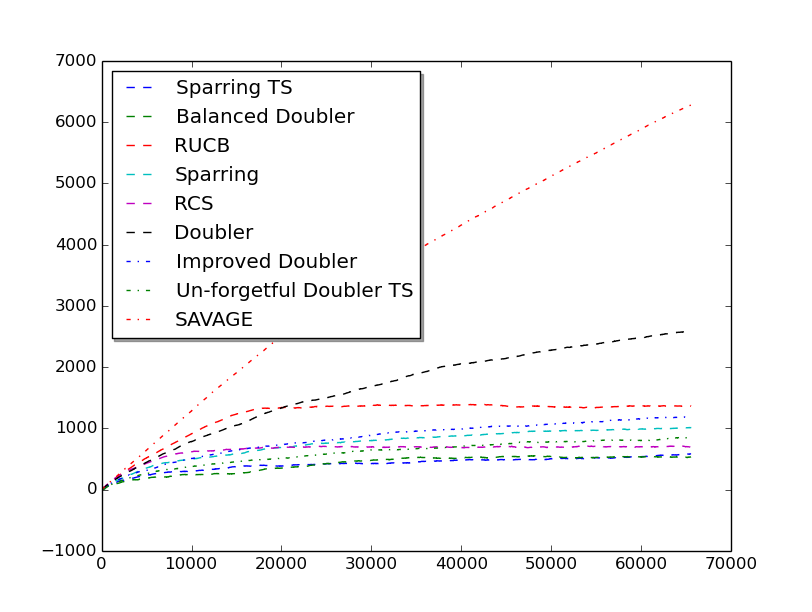
\includegraphics[scale=0.5]{figures/all_MQ2007_7arms.png}
  \caption{Utility Based Regret with 7 Arms}
\end{figure}

For a larger number of arms we can see that RCS and RUCB are outperformed by the other algorithms.

\begin{figure}[h!]
\centering
  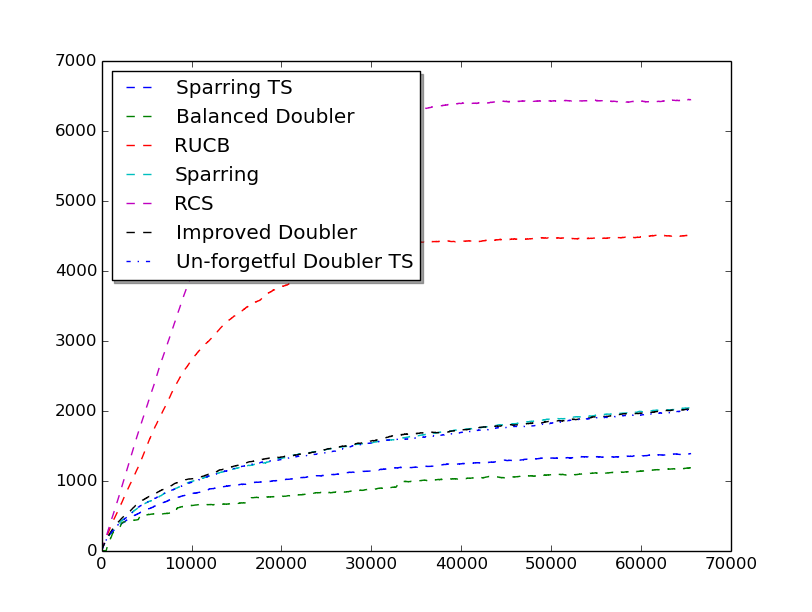
\includegraphics[scale=0.5]{figures/all_MQ2007_24arms.png}
  \caption{Utility Based Regret with 24 Arms}
\end{figure}

And for 46 arms we can see that Sparring with Thompson Sampling methods performs better than all the other algorithms.


\subsection{Sparring}

We can see the clear advantage of using the Sparring algorithm over the RCS algorithm when dealing with a large number of arms.
\begin{figure}[h!]
\centering
\begin{subfigure}{.5\textwidth}
  \centering
  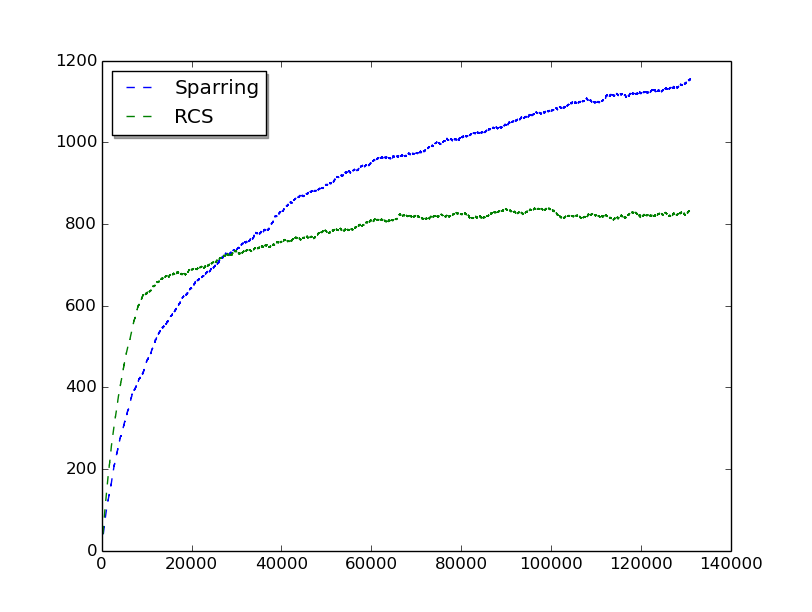
\includegraphics[scale=0.3]{figures/rcs_sparring_MQ2007_7arms.png}
  \caption{7 Arms}
  \label{fig:sub1}
\end{subfigure}%
\begin{subfigure}{.5\textwidth}
  \centering
  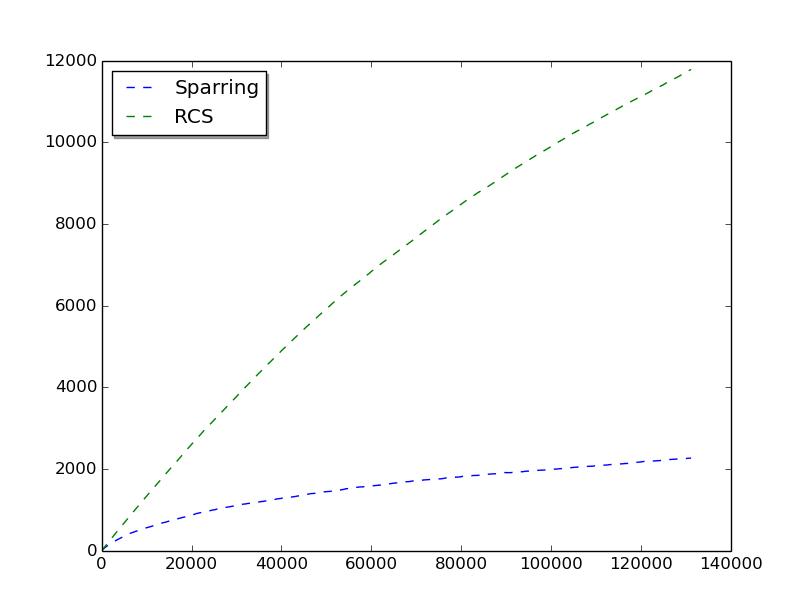
\includegraphics[scale=0.3]{figures/rcs_sparring_MQ2007_16arms.png}
  \caption{16 Arms}
  \label{fig:sub2}
\end{subfigure}
\begin{subfigure}{.5\textwidth}
  \centering
  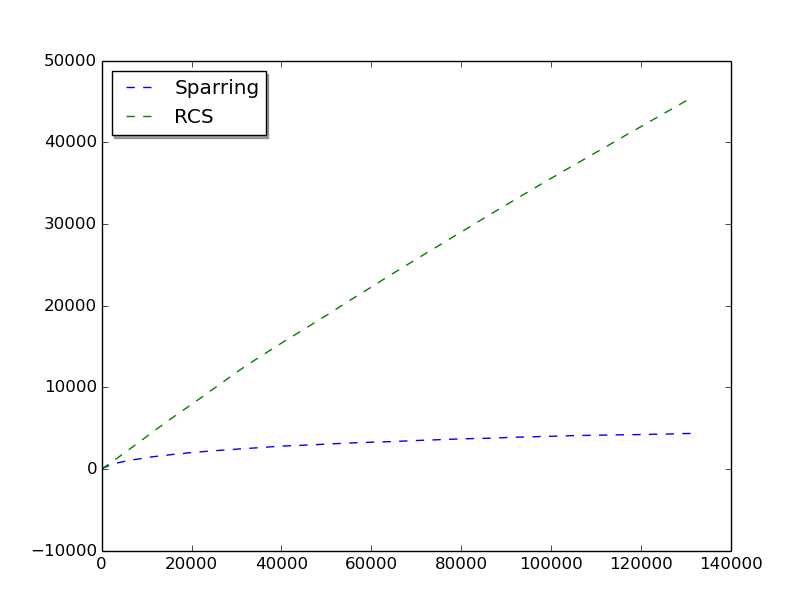
\includegraphics[scale=0.3]{figures/rcs_sparring_MQ2007_46arms.png}
  \caption{46 Arms}
  \label{fig:sub2}
\end{subfigure}
\caption{RCS Versus Sparring with Utility Based Regret}
\label{fig:test}
\end{figure}


With a small number of arms (Fig 1.) we can observe that the RCS algorithm quickly converges to the optimal arm.
\\
With a larger number of arms we can see that Sparring out-performs the RCS algorithm. 
\\
Now lets look at the general regret (as defined section 2.2). Here we used 46 arms:
\begin{figure}[h!]
  \centering
     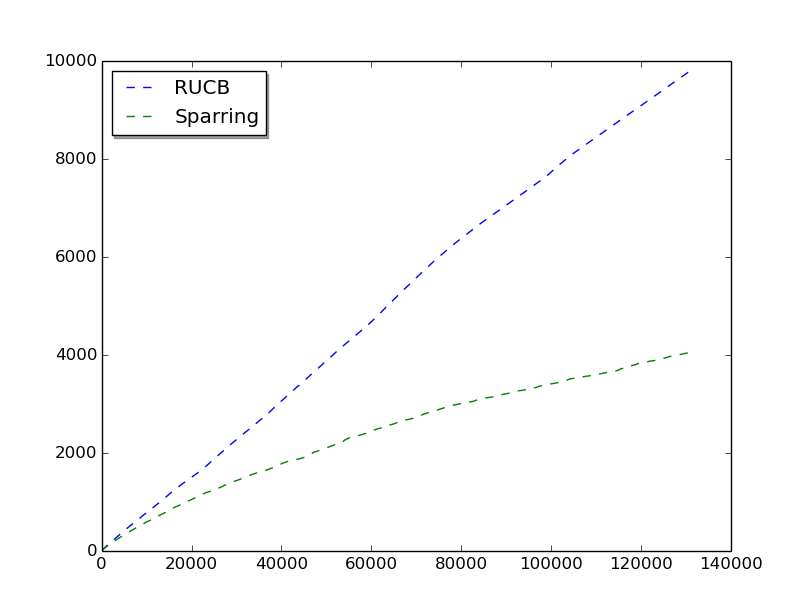
\includegraphics[scale=0.4]{figures/rcs_sparring_MQ2007_general.png} 
  \caption{RCS Versus Sparring with Preference Based Regret with 46 Arms}
\end{figure}


\newpage
\subsection{Doubler}
Now lets have a look at the Doubler algorithm using the same data set.
\begin{figure}[h!]
\centering
\begin{subfigure}{.5\textwidth}
  \centering
  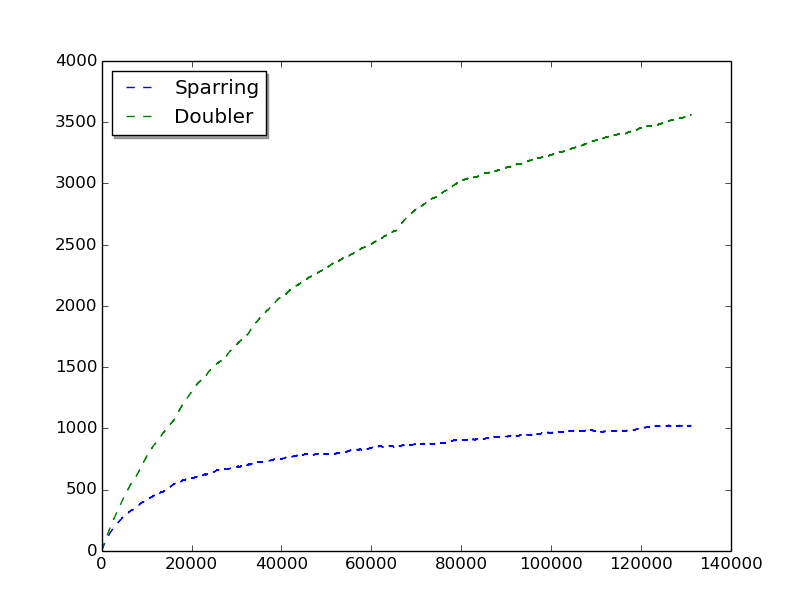
\includegraphics[scale=0.3]{figures/doubler_sparring_MQ2007_7arms.png}
  \caption{7 Arms}
  \label{fig:sub1}
\end{subfigure}%
\begin{subfigure}{.5\textwidth}
  \centering
  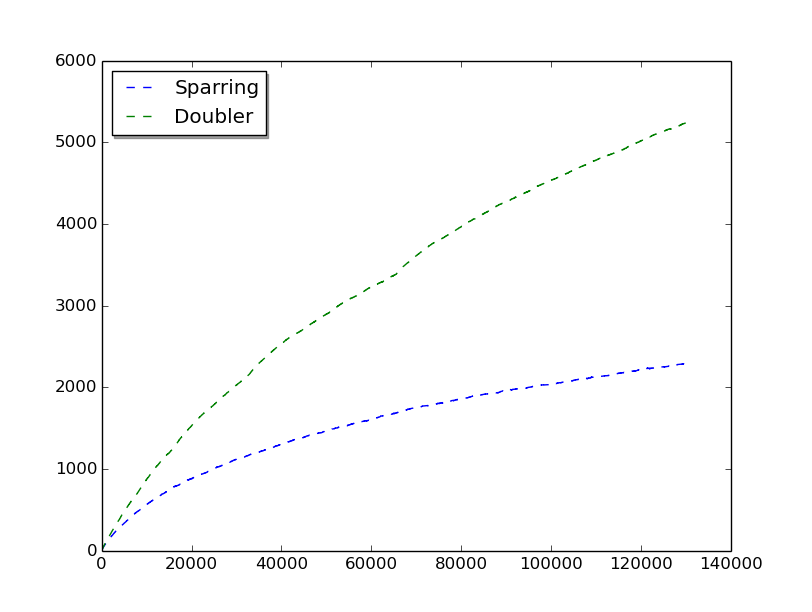
\includegraphics[scale=0.3]{figures/doubler_sparring_MQ2007_16arms.png}
  \caption{16 Arms}
  \label{fig:sub2}
\end{subfigure}
\begin{subfigure}{.5\textwidth}
  \centering
  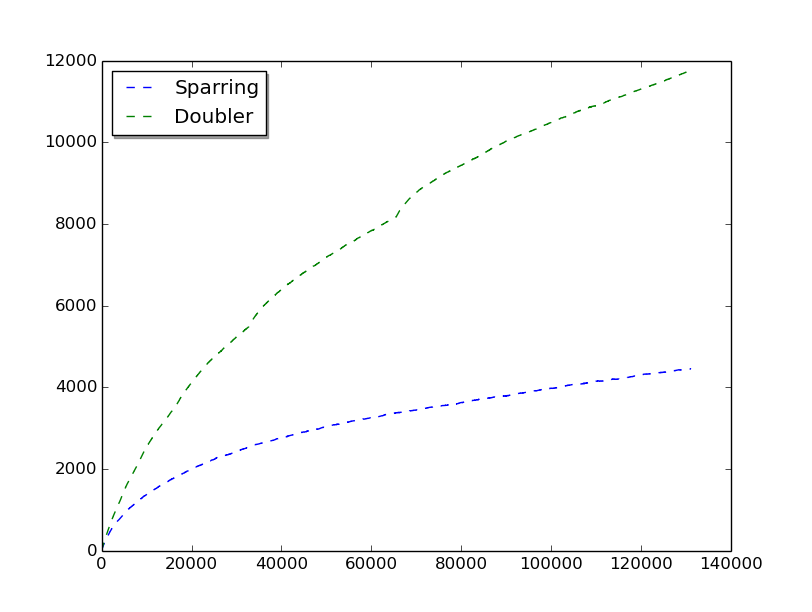
\includegraphics[scale=0.3]{figures/doubler_sparring_MQ2007_46arms.png}
  \caption{46 Arms}
  \label{fig:sub2}
\end{subfigure}
\caption{Doubler Versus Sparring with Utility Based Regret}
\label{fig:test}
\end{figure}

The general regret:
\begin{figure}[h!]
  \centering
     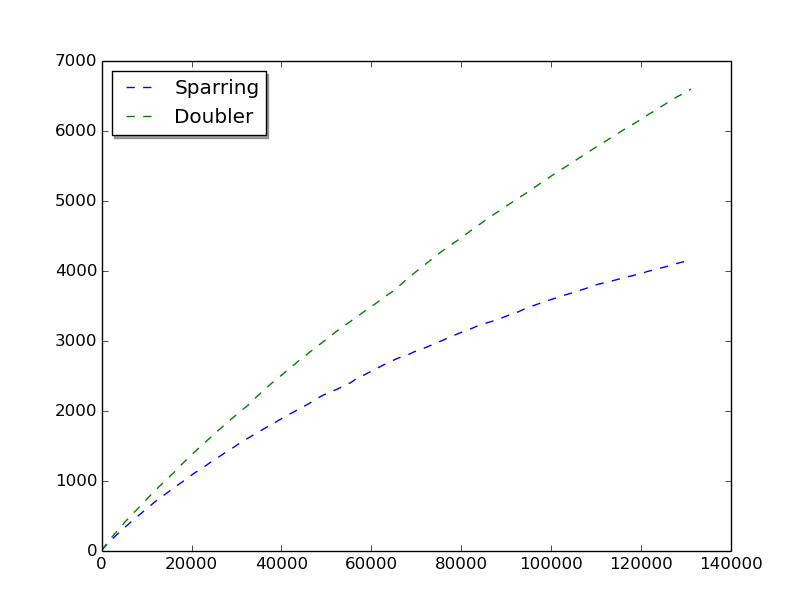
\includegraphics[scale=0.2]{figures/doubler_sparring_MQ2007_general.png} 
  \caption{Doubler Versus Sparring with Preference Based Regret with 46 Arms}
\end{figure}

\newpage
\subsection{Improved Doubler}
Now lets have a look at the Improved Doubler algorithm using the same data set.
\begin{figure}[h!]
\centering
\begin{subfigure}{.5\textwidth}
  \centering
  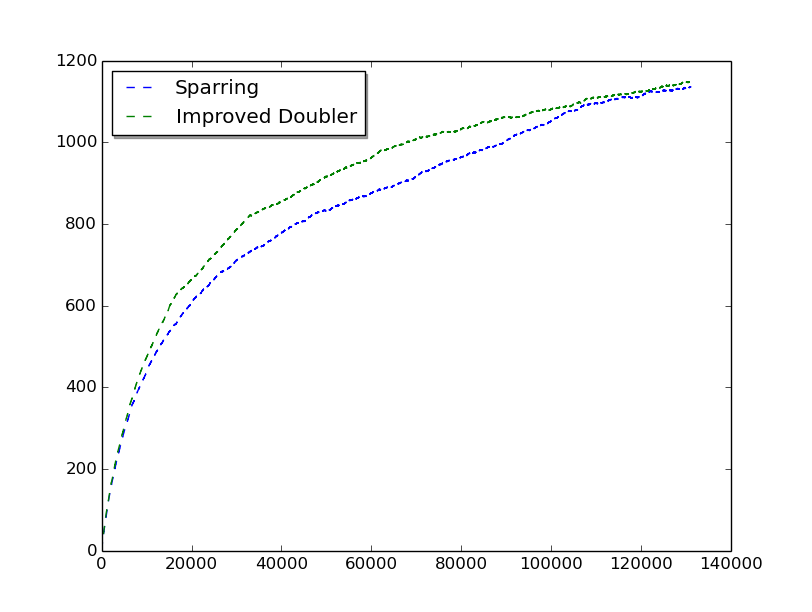
\includegraphics[scale=0.3]{figures/improved_doubler_sparring_MQ2007_7arms.png}
  \caption{7 Arms}
  \label{fig:sub1}
\end{subfigure}%
\begin{subfigure}{.5\textwidth}
  \centering
  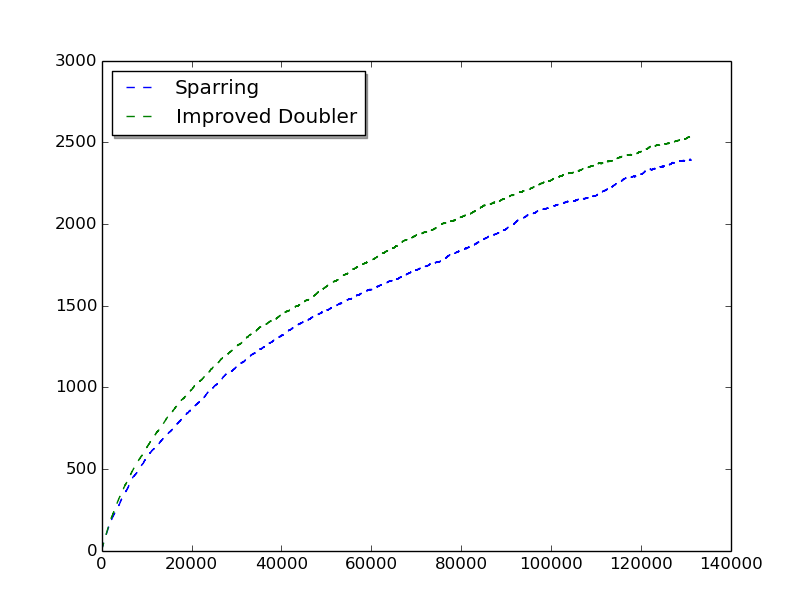
\includegraphics[scale=0.3]{figures/improved_doubler_sparring_MQ2007_16arms.png}
  \caption{16 Arms}
  \label{fig:sub2}
\end{subfigure}
\begin{subfigure}{.5\textwidth}
  \centering
  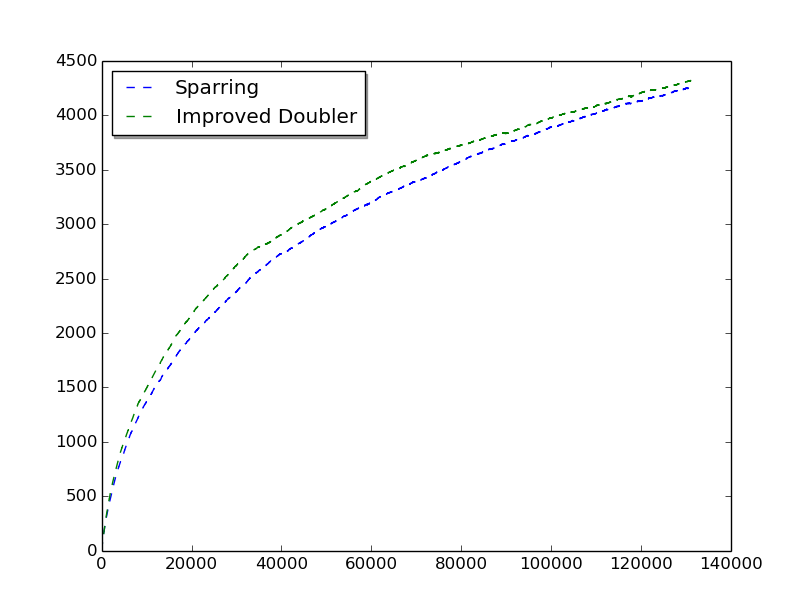
\includegraphics[scale=0.3]{figures/improved_doubler_sparring_MQ2007_46arms.png}
  \caption{46 Arms}
  \label{fig:sub2}
\end{subfigure}
\caption{Improved Doubler Versus Sparring with Utility Based Regret}
\label{fig:test}
\end{figure}

The general regret:
\begin{figure}[h!]
  \centering
     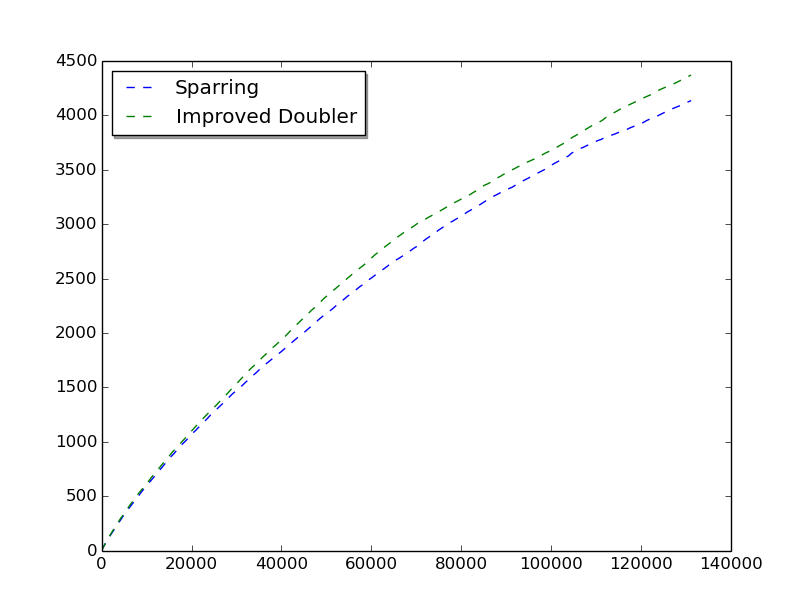
\includegraphics[scale=0.3]{figures/improved_doubler_sparring_MQ2007_general.png} 
  \caption{Improved Doubler Versus Sparring with Preference Based Regret with 46 Arms}
\end{figure}
\newpage
\subsection{Balanced Doubler}
Now lets have a look at the Balanced Doubler algorithm using the same data set.
\begin{figure}[h!]
  \centering
     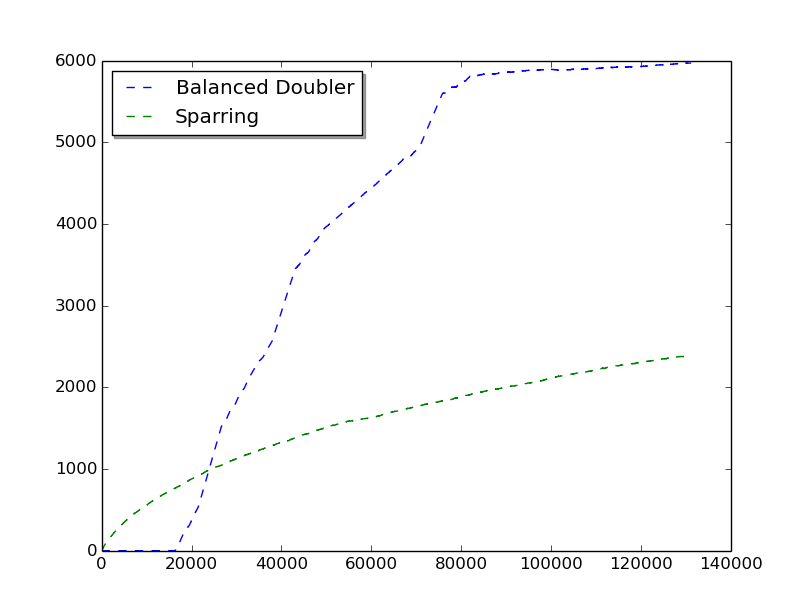
\includegraphics[scale=0.3]{figures/balanced_doubler_sparring_MQ2007_16arms.png} 
  \caption{Balanced Doubler Versus Sparring with Utility Based Regret with 16 Arms}
\end{figure}

\subsection{Thompson Sampling Doubler}
Now lets have a look at the Balanced Doubler algorithm using the same data set.
\begin{figure}[h!]
\centering
\begin{subfigure}{.5\textwidth}
  \centering
  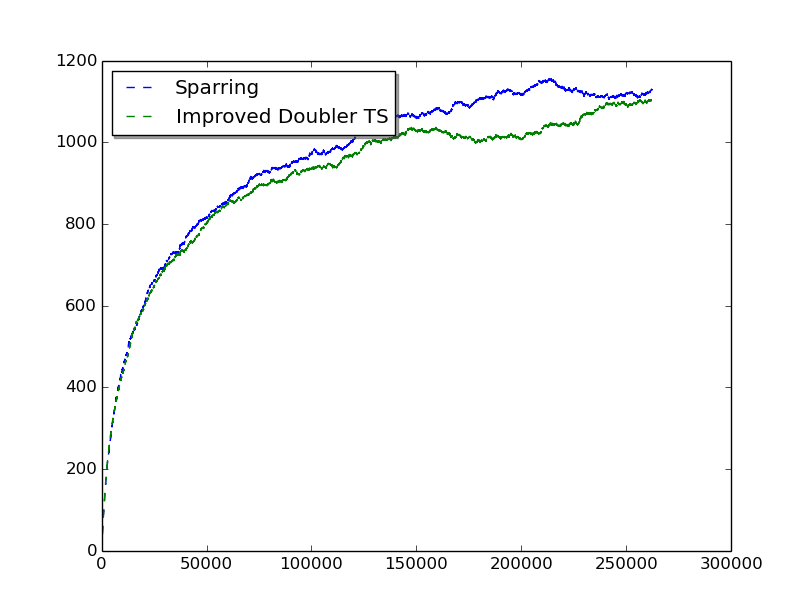
\includegraphics[scale=0.3]{figures/improved_doubler_TS_sparring_MQ2007_7arms.png}
  \caption{7 Arms}
  \label{fig:sub1}
\end{subfigure}%
\begin{subfigure}{.5\textwidth}
  \centering
  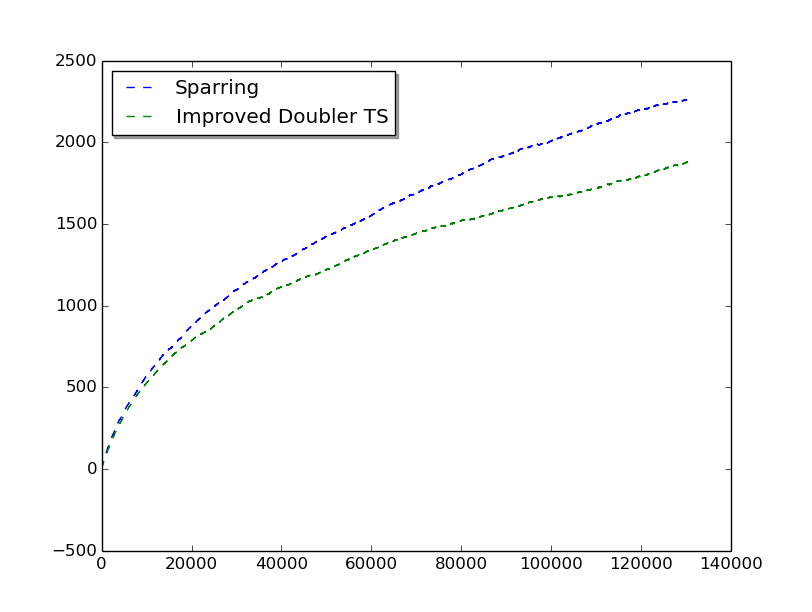
\includegraphics[scale=0.3]{figures/improved_doubler_TS_sparring_MQ2007_16arms.png}
  \caption{16 Arms}
  \label{fig:sub2}
\end{subfigure}
\begin{subfigure}{.5\textwidth}
  \centering
  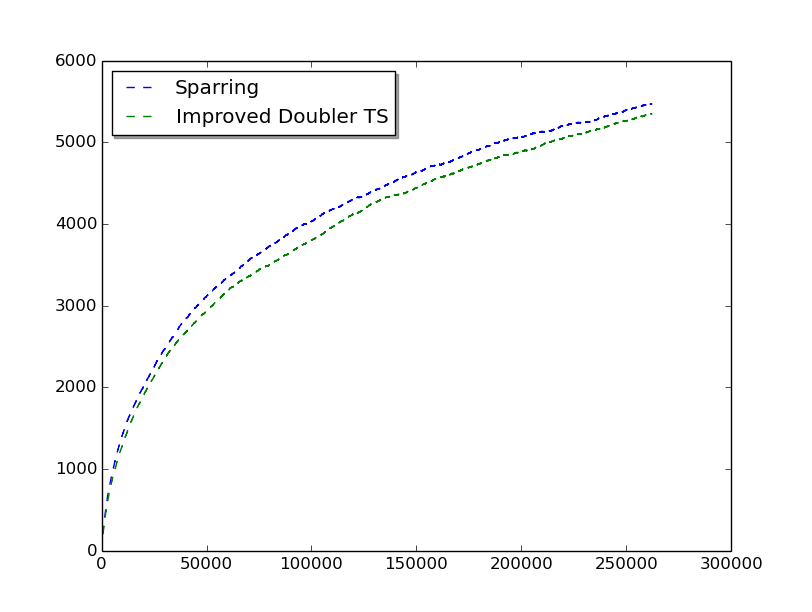
\includegraphics[scale=0.3]{figures/improved_doubler_TS_sparring_MQ2007_46arms.png}
  \caption{46 Arms}
  \label{fig:sub2}
\end{subfigure}
\caption{Improved Doubler Versus Sparring with Utility Based Regret}
\label{fig:test}
\end{figure}

The general regret:
\begin{figure}[h!]
  \centering
     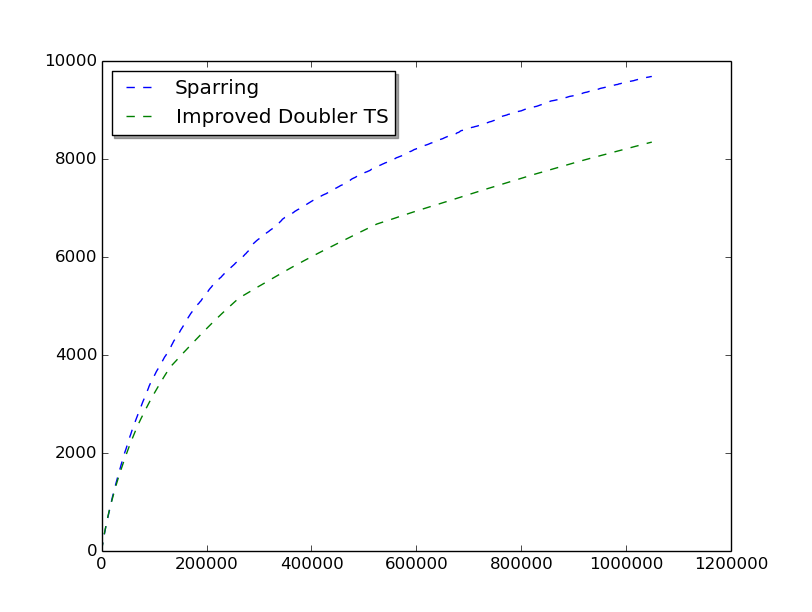
\includegraphics[scale=0.4]{figures/improved_doubler_TS_sparring_MQ2007_general.png} 
  \caption{Improved Doubler Versus Sparring with Preference Based Regret with 46 Arms}
\end{figure}

\subsection{Thompson Sampling Sparring}
And finally, lets show the results of  the sparring algorithm when using Thompson Sampling black boxes.

\begin{figure}[h!]
  \centering
     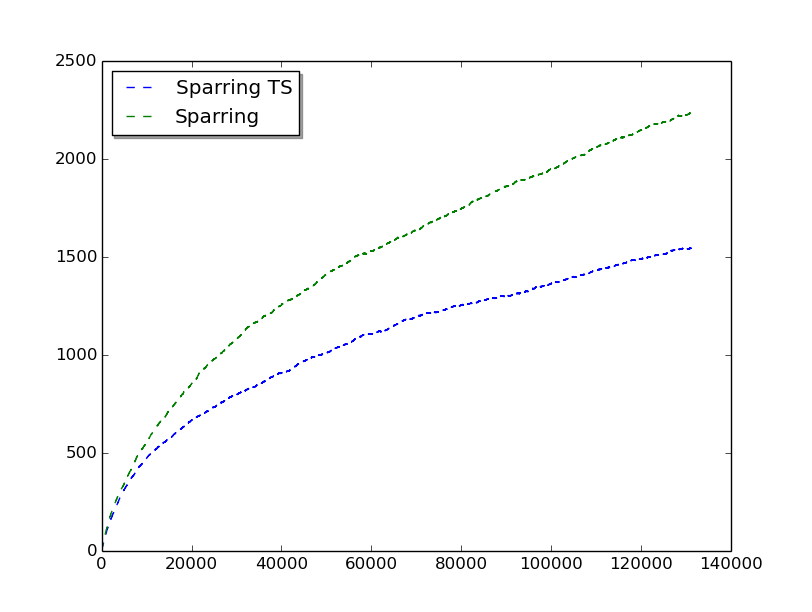
\includegraphics[scale=0.4]{figures/TS_sparring_sparring_MQ2007_16arms.png} 
  \caption{Thompson Sampling Sparring Versus Sparring with Utility Based Regret with 16 Arms}
\end{figure}

The general regret:
\begin{figure}[h!]
  \centering
     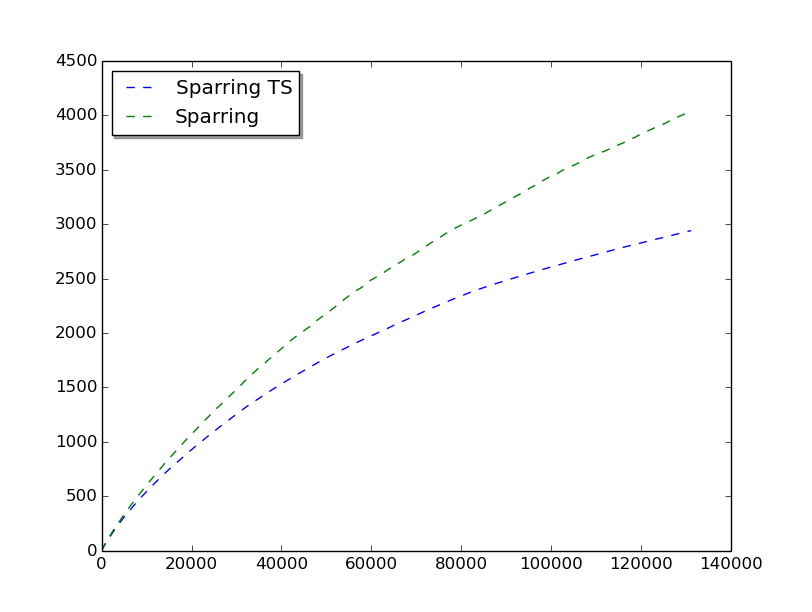
\includegraphics[scale=0.4]{figures/TS_sparring_sparring_MQ2007_general.png} 
  \caption{Thompson Sampling Sparring Versus Sparring with Preference Based Regret with 46 Arms}
\end{figure}

\end{document}
